\section{Hall Probe Investigation}
CPACs 1, 4 and 5
\hfill
\nth{11} November 2019

\subsection{History}
The Hall effect is the production of a voltage difference across an electrical conductor, transverse to an electric current in the conductor and to an applied magnetic field perpendicular to the current.
In 1879 Edwin Hall was exploring whether magnetic fields interacted with the conductors or the electric current itself, and discovered the Hall effect while he was working on his doctoral degree at Johns Hopkins University in Baltimore, Maryland.\cite{wiki:halleffect}
\par
A Hall effect sensor is a device that is used to measure the magnitude of a magnetic field. Its output voltage is directly proportional to the magnetic field strength through it. Hall sensors are commonly used to time the speed of wheels and shafts.\cite{wiki:sensor}

\subsection{Method}

\subsubsection{Method}
\begin{enumerate}
  \item Using a clamp stand, situate the Hall Probe between the two poles of the horse shoe magnet.
  \item Record the value displayed on the meter.
  \item Move the magnet 2cm further.
  \item Record the value displayed on the meter alongside the distance from the Hall Probe.
  \item Repeate steps 3 and 4  until the magnetic flux density is approximately zero.
\end{enumerate}

\subsubsection{Diagram}
\begin{figure}[H]
  \centering
  \begin{tikzpicture}[scale=0.6]
    \draw (8,0) -- (2,0) -- (2,8) -- (8,8) -- (8,6) -- (4,6) -- (4,2) -- (8,2) -- (8,0);
    \node at (3.5,0.5) {Magnet};
    \draw (9,0) rectangle (19,1);
    \node at (9.7,1.5) {Ruler};
    \foreach \x in {10,11,...,19}
    \draw (\x,0.5) -- (\x,0);
    \draw (9,3.5) rectangle (15,4.5);
    \node at (10.4,5) {Hall Probe};
  \end{tikzpicture}
  \caption{Circuit in Exp. A Method I}
\end{figure}

\subsubsection{Results}
\begin{figure}[H]
  \centering
  \pgfplotstabletypeset[
    columns={d, m},
    columns/d/.style={column type = |p{3cm},column name= distance (cm)},
    columns/m/.style={column type = |p{3cm}|,column name= magnetic flux density (mT)},
    string type
  ]{data/r_t1_a_1.txt}
  \caption{Table for Exp. A Method I}
\end{figure}

\subsubsection{Graph}
\begin{figure}[H]
  \centering
  \begin{tikzpicture}
    \begin{axis}[ylabel={distance (cm)},xlabel={magnetic flux density (mT)}]
      \addplot [mark = *] table [x=d,y=m]{data/r_t1_a_1.txt};
    \end{axis}
  \end{tikzpicture}
  \caption{Graph for Exp. A Method I}
\end{figure}

\subsubsection{Evaluation}
The resolution of the Hall Probe is 0.1mT therefore the uncertainty in the magnetic flux density is $\mp 0.05mT$.
There is a negligable uncertainty in the distance it was not measured but changed.
As no numerical value was calculated using the data there is no way to find a final uncertainty.
The precision of this experiment could be improved by using smaller angle increments to obtain more results.
The accuracy could be improved by making sure there is no external magnetic field affecting the results.

\subsubsection{Conclusion}
The shape of the graph above is observed to be inversely proporional to the cube of the distance as expected.\cite{mille:magnetic}

\subsection{Method}
\subsubsection{Method}
\begin{enumerate}
  \item Using a clamp stand, situate the Hall Probe vertically between the two poles of the horse shoe magnet.
  \item Record the value on the meter.
  \item Rotate the magnet by 10 degrees.
  \item Again record the value displayed on the meter alongside angle.
  \item Take measurements for angles up to 360 degrees.
\end{enumerate}

\subsubsection{Diagram}
\begin{figure}[H]
  \centering
  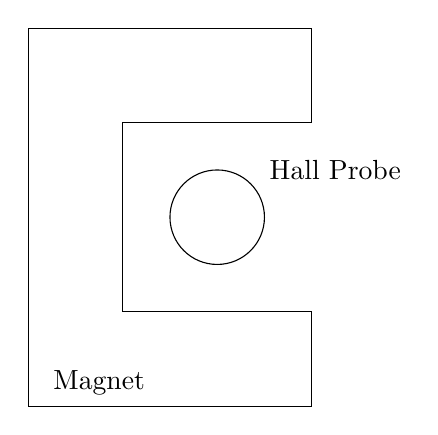
\begin{tikzpicture}[scale=0.6]
    \draw (8,0) -- (2,0) -- (2,8) -- (8,8) -- (8,6) -- (4,6) -- (4,2) -- (8,2) -- (8,0);
    \node at (3.5,0.5) {Magnet};
    \draw (6,4) circle (1);
    \node at (8.5,5) {Hall Probe};
  \end{tikzpicture}
  \caption{Diagram of Exp. A Method II}
\end{figure}

\subsubsection{Results}
\begin{figure}[H]
  \centering
  \pgfplotstabletypeset[
    columns={a, m},
    columns/a/.style={column type = |p{3cm},column name= angle ($\deg$)},
    columns/m/.style={column type = |p{3cm}|,column name= magnetic flux density (mT)},
    string type
  ]{data/r_t1_a_2.txt}
  \caption{Table for Exp. A Method II}
\end{figure}

\subsubsection{Graph}
\begin{figure}[H]
  \centering
  \begin{tikzpicture}
    \begin{axis}[ylabel={angle ($\deg$)},xlabel={magnetic flux density (mT)}]
      \addplot [mark = *] table [x=a,y=m]{data/r_t1_a_2.txt};
      \addplot [thick, red] table [x=a,y=c]{data/r_t1_a_2.txt};
    \end{axis}
  \end{tikzpicture}
  \caption{Graph for Exp. A Method II}
\end{figure}

\subsubsection{Analysis}
As our magnetic field is constant, the magnetic flux density can be defined as:
\begin{center}
  $\Phi_B=BS\cos{\theta},$
\end{center}
where $B$ is the magnitude of the magnetic field, $S$ is the area of the surface and $\theta$ is the angle between the magnetic field lines.
As shown by the red cosine curve on our graph, our data follows the same format.

\subsubsection{Evaluation}
The resolution of the Hall Probe is 0.1mT therefore the uncertainty in the magnetic flux density is $\mp 0.05mT$.
There is a negligable uncertainty in the angle it was not measured but changed.
As no numerical value was calculated using the data there is no way to find a final uncertainty.
The precision of this experiment could be improved by using smaller angle increments to obtain more results.
The accuracy could be improved by making sure there is no external magnetic field affecting the results.

\subsubsection{Conclusion}
The curve obtained by our experiment follows the expected cosine shape showing that valid results where produced.
